% IEEE conference manuscript. Evidence and build instructions: README.md.
\documentclass[conference]{IEEEtran}
\usepackage{cite}
\usepackage{amsmath,amssymb}
\usepackage{graphicx,booktabs,array}
\usepackage{balance}
\usepackage{xcolor,tikz}
\usetikzlibrary{positioning,arrows.meta}
\usepackage[hidelinks]{hyperref}
\graphicspath{{figures/}}
\newcommand{\model}{MMF-Net}
\newcommand{\bce}{N5\_bce}
\begin{document}
\title{Terrain-Conditioned Deep Neural Networks for\\Next-Day High-Flow Prediction in Sri Lanka}

\author{%
\IEEEauthorblockN{%
Ranuga Weerasekara, Heshan Nethmina, Manuja Ranathunga,\\
Vinma Wettasinghe, and Dinithi Navodya}
\IEEEauthorblockA{%
Department of Computer Science \& Engineering\\
University of Moratuwa, Moratuwa, Sri Lanka\\
\texttt{\{ranugaw.23, heshann.23, manujar.23, vinmaw.23, dinithin.23\}@cse.mrt.ac.lk}}
}

\maketitle

\begin{abstract}
This study investigates MMF-Net, a terrain-conditioned temporal
transformer for next-day high-flow prediction at 51 locations in
Sri Lanka. The model combines 14-day sequences of 33
hydrometeorological variables with nine static catchment attributes
using periodic numerical embeddings, temporal and cross-feature
attention, and feature-wise linear modulation. The prediction target
is exceedance of a location-specific discharge threshold derived
from GloFAS reanalysis, representing a high-flow proxy rather than
observed inundation. On the temporal test split, periodic embeddings
increase average precision from 0.6083 to 0.7605. The
terrain-conditioned five-seed ensemble with binary cross-entropy
training and temperature scaling achieves average precision of
0.8355, a Brier score of 0.0080, and expected calibration error of
0.0016. These findings support numerical embeddings and static
conditioning for this prediction task. Single-seed component
ablations and incomplete radar controls limit broader conclusions;
validation against observed floods remains necessary for warning
applications.
\end{abstract}
\begin{IEEEkeywords}
deep neural networks, temporal transformer, numerical embeddings,
terrain conditioning, flood prediction, Sri Lanka
\end{IEEEkeywords}

\section{Introduction}
Next-day high-flow prediction depends on recent rainfall,
antecedent wetness, river discharge, and catchment characteristics.
A neural model must capture how these variables interact over time
and how local conditions influence the response. Sri Lanka's
contrasting climatic zones provide a setting for studying these
relationships across multiple river-basin locations.

Neural networks have shown promise in rainfall--runoff modelling
and large-scale flood forecasting
\cite{kratzert2018,nearing2024}. This study examines how numerical
representations and static catchment information affect a regional
deep neural network. We investigate \model{}, which combines
periodic numerical embeddings, temporal and cross-feature
attention, and feature-wise linear modulation of static attributes.
An optional Sentinel-1 branch explores radar fusion.

Using 14-day input histories from 51 locations, we evaluate
next-day exceedance of a training-period discharge threshold.
Component ablations examine embeddings, attention, and static
conditioning; further experiments assess training objectives,
ensembling, and probability calibration.

The contribution is an empirical assessment of these established
neural components for Sri Lankan high-flow prediction. Because
the labels derive from discharge reanalysis, the results measure
prediction of a hydrological proxy. Agreement with observed
inundation and suitability for operational warnings require
separate validation.

\section{Related Work}

\subsection{Neural hydrological forecasting}
Neural rainfall-runoff models have demonstrated the value of learning
hydrological relationships from temporal sequences \cite{kratzert2018}, while
recent large-scale work has extended neural prediction to extreme flows in
ungauged watersheds \cite{nearing2024}. Local work has also applied
bidirectional LSTMs to water-level forecasting in Sri Lanka
\cite{saubhagya2025}. The present study differs in using daily high-flow
classification across multiple Sri Lankan locations with GloFAS-derived
reanalysis supervision.

\subsection{Representation and conditioning}
Transformers use self-attention to model temporal relationships
\cite{vaswani2017}. Gorishniy \emph{et al.} showed that numerical feature
embeddings, including periodic embeddings, can improve deep tabular models
\cite{gorishniy2022}. \model{} applies periodic embeddings before temporal
encoding and uses FiLM conditioning \cite{perez2018} to incorporate static
terrain, climatic and network attributes.

River topology can also be incorporated through graph models, but its benefit
is not guaranteed. Kirschstein and Sun found no improvement from supplied
river topology in their neural forecasting experiments \cite{kirschstein2024}.
\model{} uses shared weights across locations without inter-location
message passing.

\subsection{Evaluation and probability quality}
Focal loss addresses class imbalance by reducing the influence of easy
examples \cite{lin2017}, while deep ensembles and temperature scaling provide
approaches to uncertainty estimation and calibration
\cite{lakshminarayanan2017,guo2017}. Precision-recall analysis is particularly
useful for imbalanced event prediction \cite{saito2015}, while temporal
dependence requires evaluation procedures that respect the data structure
\cite{roberts2017}. These considerations guide the evaluation and
interpretation of \model{}.

\section{Study Data and Prediction Task}
\label{sec:data}

\subsection{Spatial Coverage and Data Provenance}
The study covers 51 node locations grouped into 16 hydrological basins/areas in Sri Lanka (including the Colombo metropolitan area), distributed across the wet (31 nodes), dry (13 nodes), and intermediate (7 nodes) climatic zones. Spatial graph representations comprise 35 curated upstream-to-downstream flow links and 204 spatial links for graph-based architectures (Fig.~\ref{fig:map}). Gauge-measured discharge is not used directly.

\begin{figure}[t]
\centering
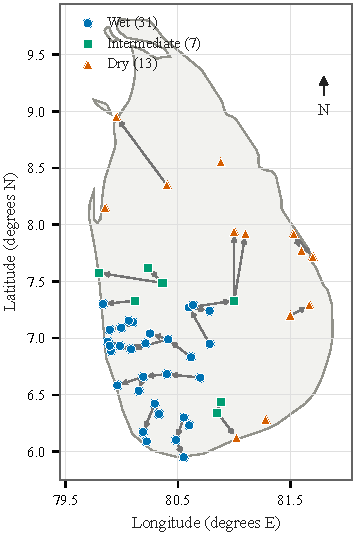
\includegraphics[width=0.45\linewidth]{fig_study_area.pdf}
\caption{Study locations and curated links, coloured by climatic zone.
Country outline: Natural Earth.}
\label{fig:map}
\end{figure}

Daily meteorological and soil-wetness attributes are sourced from NASA POWER \cite{power}, supplemented by cached Open-Meteo Archive precipitation and GloFAS reanalysis discharge via the Open-Meteo Flood API \cite{harrigan2020,openmeteo}.

The feature space comprises:
\begin{itemize}
    \item \textbf{33 Dynamic Inputs:} Rainfall and antecedent precipitation (11), temperature, humidity, wind, and radiation (7), soil wetness (6), and discharge metrics including rolling means, recent changes, seasonal anomalies, and empirical percentiles (9).
    \item \textbf{9 Static Inputs:} Elevation, climatic-zone indicators (3), network-position indicators (4), and a drainage proxy ($\log$ mean-training-discharge).
\end{itemize}

Heavy-tailed dynamic features are transformed using signed $\log(1+|x|)$ followed by z-score standardization. Missing normalized values are zero-imputed (representing the training mean).

\subsection{Targets and Episode Definition}
Let $Q_{n,t}$ denote reanalysis discharge at location $n$ on day $t$. The location-specific high-flow threshold $\tau_n$ is defined as the 98th empirical percentile of historical daily discharge through 2017:
\begin{align}
\tau_n &= \operatorname{quantile}_{0.98}\{Q_{n,t}: t \leq \text{2017-12-31}\}, \\
s_{n,t} &= \mathbf{1}[Q_{n,t} \geq \tau_n], \qquad y^{(1)}_{n,t} = s_{n,t+1}
\end{align}
where $y^{(1)}_{n,t}$ serves as the primary binary target for next-day high-flow prediction.

Auxiliary targets include multi-day exceedance $y^{(h)}_{n,t} = \max_{k=1,\ldots,h} s_{n,t+k}$ for $h \in \{2, 3\}$, event onset $y^{(o)}_{n,t} = (1 - s_{n,t})s_{n,t+1}$, and regression heads predicting the next-day discharge percentile and 3-day maximum discharge z-score.

Proxy episodes are defined per node by grouping consecutive positive state days ($s_{n,t}=1$) separated by at most a one-day gap.

\subsection{Dataset Scope}
The primary DNN input sequence is truncated at 31 December 2024. The full catalog contains 1,469 proxy episodes (1,464 starting in 2003--2024) split across training, validation, and testing periods (Fig.~\ref{fig:episodes}).

\begin{figure}[htbp]
\centering
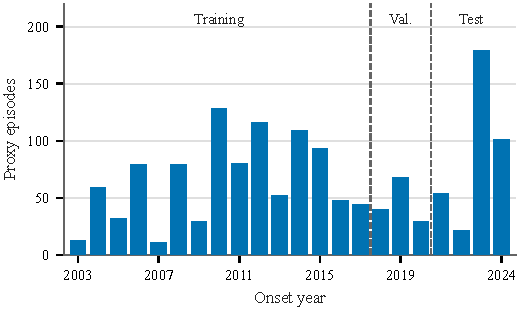
\includegraphics[width=0.85 \linewidth]{fig_episode_profile.pdf}
\caption{Annual distribution of node-level proxy episode onsets (2003--2024) across experimental temporal splits.}
\label{fig:episodes}
\end{figure}

\section{Deep Neural Network Method}
\label{sec:method}
 
\subsection{Numerical and temporal representation}
Each prediction uses a 14-day, 33-variable history per node,
$\mathbf{X}_{n,t}\in\mathbb{R}^{14\times33}$, with nodes processed
independently via the batch dimension. Each scalar feature $j$ is embedded
using a periodic-linear-ReLU (PLR) representation with trainable sine/cosine
frequencies $\mathbf{c}_j\in\mathbb{R}^{8}$:
\begin{equation}
\mathbf{e}_j(x)=\operatorname{ReLU}\!\left(
\mathbf{W}_j[\sin(2\pi\mathbf{c}_j x)\Vert
\cos(2\pi\mathbf{c}_j x)]+\mathbf{b}_j\right).
\end{equation}
Daily embeddings are concatenated, projected to 128 dimensions, and passed
(with position and classification tokens) through three pre-LN transformer
blocks (4 heads, feed-forward width 256, dropout 0.2), yielding the temporal
representation $\mathbf{h}^{T}$.
 
\subsection{Cross-feature attention and static conditioning}
A parallel branch averages embeddings over time, projects each feature to a
128-dimensional token, and applies a one-layer transformer to obtain
$\mathbf{h}^{F}$. The branches merge as
\begin{equation}
\mathbf{h}=\operatorname{LN}(\mathbf{h}^{T}+\mathbf{h}^{F}).
\end{equation}
A 9-dimensional static vector $\mathbf{s}_n$ supplies the scale and shift
vectors $\gamma_n$ and $\beta_n$ through a zero-initialised FiLM layer:
\begin{equation}
\widetilde{\mathbf{h}}=\operatorname{LN}
 [\mathbf{h}\odot(1+\gamma_n)+\beta_n].
\end{equation}
A fusion MLP (widths 192, 128) and shared head (widths 256, 128) produce the
classification and regression outputs (Fig.~\ref{fig:architecture}).
 
\begin{figure}[t]
\centering
\resizebox{\columnwidth}{!}{%
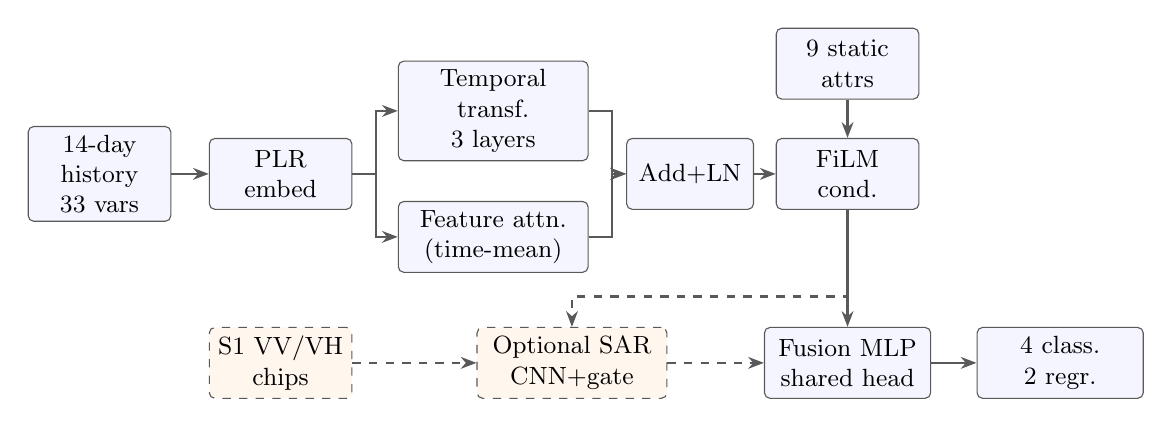
\begin{tikzpicture}[font=\small,
 b/.style={draw=black!65,rounded corners=2pt,align=center,minimum height=9mm,
 text width=1.6cm,inner sep=3pt,fill=blue!4},
 a/.style={-{Stealth[length=2mm]},thick,black!65}]
\node[b] (x) at (0,0) {14-day history\\33 vars};
\node[b] (e) at (2.3,0) {PLR embed};
\node[b,text width=2.2cm] (t) at (5.0,0.8) {Temporal transf.\\3 layers};
\node[b,text width=2.2cm] (f) at (5.0,-0.8) {Feature attn.\\(time-mean)};
\node[b,text width=1.4cm] (m) at (7.5,0) {Add+LN};
\node[b] (film) at (9.5,0) {FiLM cond.};
\node[b] (s) at (9.5,1.4) {9 static attrs};
\node[b,dashed,fill=orange!7,text width=2.2cm] (sar) at (6.0,-2.4) {Optional SAR CNN+gate};
\node[b,dashed,fill=orange!7] (img) at (2.3,-2.4) {S1 VV/VH chips};
\node[b,text width=1.9cm] (head) at (9.5,-2.4) {Fusion MLP\\shared head};
\node[b,text width=1.9cm] (out) at (12.2,-2.4) {4 class.\\2 regr.};
\draw[a] (x) -- (e);
\draw[a] (e.east) -- ++(0.3,0) |- (t.west);
\draw[a] (e.east) -- ++(0.3,0) |- (f.west);
\draw[a] (t.east) -- ++(0.3,0) |- (m.west);
\draw[a] (f.east) -- ++(0.3,0) |- (m.west);
\draw[a] (m) -- (film); \draw[a] (s) -- (film);
\draw[a] (film) -- (head);
\draw[a,dashed] (film.south) -- ++(0,-1.1) -| (sar.north);
\draw[a,dashed] (img) -- (sar);
\draw[a,dashed] (sar) -- (head); \draw[a] (head) -- (out);
\end{tikzpicture}}
\caption{Model data flow: parallel temporal/feature branches merge and are
conditioned on static attributes; optional radar fusion (dashed) feeds the
shared head. No graph message passing is used.}
\label{fig:architecture}
\end{figure}
 
\subsection{Optional radar branch}
An optional CNN maps Sentinel-1 VV/VH chips to an embedding $\mathbf{v}$.
A learned gate (bias initialised to $-3$) combines it with the tabular state,
using a binary presence indicator $m$ and image age $a$ in days:
\begin{align}
\mathbf{g}&=\sigma\{\operatorname{MLP}
 [\widetilde{\mathbf{h}}\Vert\mathbf{v}\Vert m\Vert(a/30)]\},\\
\mathbf{h}^{S}&=\operatorname{LN}
 (\widetilde{\mathbf{h}}+m\,\mathbf{g}\odot\mathbf{W}_v\mathbf{v}).
\end{align}
Here, $\sigma$ is the sigmoid function and $\mathbf{W}_v$ projects the
image embedding; absent frames contribute zero because $m=0$.
A simpler scalar variant appends four image-derived summaries instead.
Imagery is available for only 9 of 51 nodes, and no verified pretrained
checkpoint exists, so this branch is not a validated pretrained-radar result.
 
\subsection{Multi-task optimisation and calibrated inference}
Training minimises masked BCE across four classification heads (weights
$1.0,0.3,0.3,0.5$) plus weighted Huber loss over two regressions (0.2); an
alternative \texttt{focal\_conf} loss instead jointly adjusts class
weighting, focal focusing ($\alpha=0.75$, $\gamma=2$), and label confidence.
Optimisation uses AdamW ($10^{-3}$ lr, $10^{-4}$ decay, cosine schedule with
5 warmup epochs, $\leq$60 epochs, gradient clipping at 1.0, patience-10
early stopping). At inference, five-seed probability averages are temperature
calibrated,
\begin{equation}
p_{\mathrm{cal}}=\sigma\!\left[\operatorname{logit}(\bar p)/T\right],
\end{equation}
where $\bar p$ is the mean predicted probability and $T>0$ is the
temperature. Validation-based selection is described below.

\section{Experimental Design}

\subsection{Configuration and Ablations}

\begin{table}[t]
\caption{Experimental configuration.}
\label{tab:settings}
\centering
\footnotesize
\begin{tabular}{@{}p{0.36\columnwidth}p{0.58\columnwidth}@{}}
\toprule
Setting & Value \\
\midrule
Training period & 2003--2017 \\
Validation period & 2018--2020 \\
Test period & 2021--2024 \\
Input window & 14 days; 33 dynamic and 9 static features \\
Transformer layers & 3 temporal; 1 cross-feature \\
Hidden dimension / heads & 128 / 4 \\
Batch size & 32; SAR CNN: 8 \\
Optimiser / epochs & AdamW; maximum 60 \\
Seeds & N0--N4: 1; ensemble variants: 5 \\
\bottomrule
\end{tabular}
\end{table}

Table~\ref{tab:settings} summarises the experimental settings.
N0--N3 progressively introduce periodic numerical embeddings,
cross-feature attention and FiLM conditioning. N4 evaluates
combined focal and label-confidence weighting. N5 and
\bce{} use five-seed ensembles with temperature scaling
under the weighted objective and binary cross-entropy,
respectively. N6 variants explore SAR fusion.
Single-seed ablations are interpreted descriptively.
Earlier graph-network and conventional baseline results
use a different data extent and are reported separately.

\subsection{Evaluation}

Checkpoints are selected using validation episode average
precision (AP). Calibration and F1-based threshold selection
use validation data only and are frozen for testing.
We report node-day AP, Brier score, expected calibration
error (ECE) using 15 equal-width bins, probability of detection
(POD), false-alarm ratio (FAR), and critical success
index (CSI):
\begin{equation}
\begin{aligned}
\mathrm{POD} &= \frac{TP}{TP+FN}, \\
\mathrm{FAR} &= \frac{FP}{TP+FP}, \\
\mathrm{CSI} &= \frac{TP}{TP+FP+FN}.
\end{aligned}
\end{equation}
Here, $TP$, $FP$ and $FN$ denote true positives,
false positives and false negatives, respectively.

Episode detection measures the fraction of episodes with
an alarm during the preceding seven days. Episode AP
uses the maximum pre-onset probability, with flood-free
node-weeks as negatives. This retrospective measure
does not establish seven-day forecasting skill.
Detection rates are interpreted alongside FAR because
models use different validation-selected thresholds.

\section{Results}

\subsection{Neural representation and static conditioning}
Table~\ref{tab:ablation} reports the recorded \model{} results. PLR
embeddings raise AP from 0.6083 to 0.7605; feature attention raises it
further to 0.7738; static FiLM conditioning raises it to 0.8269. This
supports flexible scalar representations and location-dependent
conditioning, but the FiLM contrast does not isolate elevation from the
other static inputs (drainage proxy, zone, position) fed to the same module.
N0--N4 use one seed each, so their differences describe these specific runs,
not statistically established component effects.

\begin{table}[t]
\caption{Main DNN results on the temporal test split.}
\label{tab:ablation}
\centering\footnotesize
\begin{tabular}{@{}llrrrr@{}}
\toprule
ID & Configuration & AP & ECE & FAR & Params \\
\midrule
N0 & Linear embeddings & .6083 & .0024 & .412 & .551 \\
N1 & + PLR & .7605 & .0053 & .325 & .555 \\
N2 & + feature attention & .7738 & .0056 & .313 & .693 \\
N3 & + static FiLM & .8269 & .0032 & .110 & .711 \\
N4 & + focal/confidence & .7592 & .0525 & .138 & .711 \\
N5 & N4, ensemble + TS & .7846 & .0043 & .145 & .711 \\
\bce{} & N3, ensemble + TS & \textbf{.8355} & .0016 & .120 & .711 \\
\midrule
N6-sc & SAR scalars, focal/conf. & .7284 & .0055 & .344 & .719 \\
N6-gat & SAR CNN, focal/conf. & .8310 & .0066 & .107 & 11.967 \\
\bottomrule

\end{tabular}\par
\vspace{4pt}
\noindent
\parbox[t]{\columnwidth}{%
  \scriptsize\raggedright
  TS: temperature scaling; focal/conf.: focal/confidence objective.
  N0--N4: one seed;
  others: five. Params: trainable millions/member.
  Bold = largest recorded AP, not significance.
  Source: model-2 snapshot, 10--11 Aug 2026.
}
\end{table}

\subsection{Objective, ensemble and calibration}
Replacing BCE with the combined focal/confidence objective moves N3's AP
from 0.8269 to 0.7592 and ECE from 0.0032 to 0.0525. In the ensemble
comparison, \bce{} (AP 0.8355, ECE 0.0016) outperforms N5 (0.7846, 0.0043),
favouring BCE here without establishing that focal loss is generally
unsuitable, or which term in the combined weighting drives the change. The
\bce{} ensemble records Brier 0.0080 and CSI 0.561, exceeding N3's AP by
0.0086. Temperature scaling preserves ranking, so it does not explain
the AP gain; separate effects on probability quality are not established. Reliability
curves and event-stratified calibration would be more informative than ECE
alone but are not recoverable from the available results.

\subsection{Radar fusion and model size}
Scalar radar: AP 0.7284. Gated CNN: AP 0.8310, versus 0.7846
(image-free focal/confidence ensemble) and 0.8355 (image-free BCE ensemble)
- mixed evidence, since the CNN beats the focal/confidence family but not
the strongest image-free result; differing objectives, batch sizes,
uncertain pretraining, and limited node coverage prevent attributing the
gap to radar alone. \bce{} uses $\sim$0.711M parameters/member vs.\ 11.967M
for N6-gat; a five-member image-free ensemble totals $\sim$3.56M parameters
and needs five forward passes. Parameter counts include gradient-enabled
weights, so checkpoint freeze status must accompany any size comparison;
latency and energy were not measured.

\subsection{Detection at recorded operating points}
Under the seven-day rule: N2 detects 0.423 of episodes at FAR 0.313; N3
detects 0.197 at FAR 0.110; \bce{} detects 0.220 at FAR 0.120. Each point
reflects both model and validation-selected threshold; these are not points
on a shared operating curve and do not establish preference at a fixed
false-alarm budget.

\subsection{Historical references and split diagnostics}
\begin{table}[t]
\caption{Historical references (2 Aug 2026); panel extent differs from
Table~\ref{tab:ablation}. Dashes: unavailable.}
\label{tab:legacy}
\centering\footnotesize
\begin{tabular}{@{}lrrrr@{}}
\toprule
Reference & AP & Brier & FAR & Detection \\
\midrule
Persistence & .590 & - & .231 & .223 \\
Climatology & .108 & - & .882 & .515 \\
Discharge percentile & .816 & - & .231 & .223 \\
LightGBM & .8496 & .0076 & .080 & .161 \\
GRU only (M0) & .598 & .0137 & .441 & .262 \\
TF-STGNN (M3) & .704 & .0135 & .342 & .380 \\
\bottomrule
\end{tabular}
\end{table}

Discharge-percentile AP ($\approx$0.816) indicates substantial persistence
in the next-day target; LightGBM reaches 0.8496 on its own historical panel
(Table~\ref{tab:legacy}). These motivate strong references for a matched
rerun but do not establish a DNN-vs-tree ordering on an identical test set;
comparing graph-based M3 to \model{} would also change encoder and panel,
not just graph structure. M3 diagnostics show AP 0.704 (temporal split) vs.\
0.905 (random split), with seven-day detection dropping from 0.380 to 0.089
- the random protocol interleaves node-days and can remove pre-onset alarm
opportunities, so this shows split sensitivity without isolating a causal
loss of warning skill or proving memorisation. The Gin holdout (AP 0.840)
tests spatial transfer on four nodes (training elsewhere spans later dates)
and is not a future-time test; strict spatial evaluation would also require
revisiting held-out-node preprocessing statistics and graph access.

\section{Practical Interpretation and Limitations}

\subsection{Operational Relevance}
MMF-Net could support river monitoring by presenting
high-flow probabilities alongside observed water levels
and rainfall. However, reanalysis-derived targets represent
a hydrological proxy, and operational warning capability
has not been validated. Effective lead time depends on
actual input availability, including publication delays
and radar acquisition times.

\subsection{Validation and Reproducibility}
The high-flow proxy activates in seven of ten documented
flood windows during 2003--2024, missing the May 2003,
June 2014 and May 2017 events. This limited label-agreement
check does not measure DNN warning accuracy. Independent
gauge and inundation observations are needed to assess
missed events and false alarms.

Future targets can cross temporal split boundaries and
must be excluded in a controlled rerun. Exact sample
counts, run configurations and prediction archives are
also required for reproducibility. Since the test set
informed model development, confirmation requires an
independent evaluation period.

\subsection{Further Evaluation}
Repeated DNN ablations should hold data, seeds and
training settings fixed to isolate the effects of
embeddings, FiLM, graph structure and radar fusion.
Operational evaluation should use validation-selected
thresholds under a stated false-alarm constraint,
report realised test FAR, and assess horizon-aligned
event detection. Calibration and uncertainty estimates
should account for temporal and cross-node dependence.

\section{Conclusion}
This study examines a terrain-conditioned deep neural network for next-day
high-flow prediction at Sri Lankan river-basin locations. Recorded ablations
show improvements after periodic numerical embeddings and static FiLM
conditioning are introduced, while the BCE ensemble attains the highest
recorded \model{} AP of 0.8355. Radar results remain exploratory and the
available experiments do not isolate the value of graph structure. The findings
support further controlled study of neural representation and fusion.
Establishing a practical warning benefit requires independent flood observations,
issue-time input replay and matched evaluation of onset detection, false alarms
and probability calibration.

\balance
\begin{thebibliography}{00}
\bibitem{kratzert2018} F. Kratzert, D. Klotz, C. Brenner, K. Schulz, and
M. Herrnegger, ``Rainfall-runoff modelling using Long Short-Term Memory (LSTM)
networks,'' \emph{Hydrol. Earth Syst. Sci.}, vol. 22, pp. 6005-6022, 2018,
doi: 10.5194/hess-22-6005-2018.
\bibitem{nearing2024} G. Nearing \emph{et al.}, ``Global prediction of extreme
floods in ungauged watersheds,'' \emph{Nature}, vol. 627, pp. 559-563, 2024,
doi: 10.1038/s41586-024-07145-1.
\bibitem{saubhagya2025} S. Saubhagya, C. Tilakaratne, P. Lakraj, and
M. Mammadov, ``A fusion of deep learning and time series regression for flood
forecasting: An application to the Ratnapura area based on the Kalu river basin
in Sri Lanka,'' \emph{Forecasting}, vol. 7, no. 2, art. 29, 2025,
doi: 10.3390/forecast7020029.
\bibitem{vaswani2017} A. Vaswani \emph{et al.}, ``Attention is all you need,''
in \emph{Advances in Neural Information Processing Systems}, vol. 30, 2017.
\bibitem{gorishniy2022} Y. Gorishniy, I. Rubachev, and A. Babenko, ``On
embeddings for numerical features in tabular deep learning,'' in
\emph{Advances in Neural Information Processing Systems}, vol. 35, 2022.
\bibitem{perez2018} E. Perez, F. Strub, H. de Vries, V. Dumoulin, and
A. Courville, ``FiLM: Visual reasoning with a general conditioning layer,''
in \emph{Proc. AAAI}, vol. 32, no. 1, 2018,
doi: 10.1609/aaai.v32i1.11671.
\bibitem{kirschstein2024} N. Kirschstein and Y. Sun, ``The merit of river
network topology for neural flood forecasting,'' in \emph{Proc. ICML},
PMLR vol. 235, pp. 24713-24725, 2024.
\bibitem{lin2017} T.-Y. Lin, P. Goyal, R. Girshick, K. He, and P. Doll\'{a}r,
``Focal loss for dense object detection,'' in \emph{Proc. ICCV},
pp. 2980-2988, 2017.
\bibitem{lakshminarayanan2017} B. Lakshminarayanan, A. Pritzel, and C. Blundell,
``Simple and scalable predictive uncertainty estimation using deep ensembles,''
in \emph{Advances in Neural Information Processing Systems}, vol. 30, 2017.
\bibitem{guo2017} C. Guo, G. Pleiss, Y. Sun, and K. Q. Weinberger,
``On calibration of modern neural networks,'' in \emph{Proc. ICML},
PMLR vol. 70, pp. 1321-1330, 2017.
\bibitem{saito2015} T. Saito and M. Rehmsmeier, ``The precision-recall plot is
more informative than the ROC plot when evaluating binary classifiers on
imbalanced datasets,'' \emph{PLOS ONE}, vol. 10, no. 3, art. e0118432, 2015,
doi: 10.1371/journal.pone.0118432.
\bibitem{roberts2017} D. R. Roberts \emph{et al.}, ``Cross-validation strategies
for data with temporal, spatial, hierarchical, or phylogenetic structure,''
\emph{Ecography}, vol. 40, no. 8, pp. 913-929, 2017,
doi: 10.1111/ecog.02881.
\bibitem{power} NASA POWER, ``Meteorology: Data sources and methodology.''
[Online]. Available: \url{https://power.larc.nasa.gov/docs/methodology/meteorology/}.
Accessed: Sep. 8, 2026.
\bibitem{harrigan2020} S. Harrigan \emph{et al.}, ``GloFAS-ERA5 operational
global river discharge reanalysis 1979-present,'' \emph{Earth Syst. Sci. Data},
vol. 12, pp. 2043-2060, 2020, doi: 10.5194/essd-12-2043-2020.
\bibitem{openmeteo} Open-Meteo, ``Flood API.'' [Online]. Available:
\url{https://open-meteo.com/en/docs/flood-api}. Accessed: Sep. 8, 2026.
\end{thebibliography}
\end{document}
